Deciding whether to invest in on-premise hardware or move to the cloud for deep learning (DL) is not easy.
Wanting to scale existing infrastructure means paying upfront, as combining cloud and on-premise is not an option with popular DL frameworks due to needing a dedicated high-bandwidth interconnect.
To enabled model- and data-parallelism, current state-of-the-art accelerators have bandwidths of 900~GB/s for intra-node~\cite{elster2022nvidia} and 25~Gb/s for inter-node setups~\cite{sergeev2018horovod,li2020pytorch}. 
% GC: https://cloud.google.com/vpc/network-pricing#footnote-2
% AWS: https://aws.amazon.com/ec2/pricing/on-demand/
% Azure: https://azure.microsoft.com/en-us/pricing/details/bandwidth/
\begin{table}[]
\begin{center}
\scalebox{0.95}{
\begin{tabular}{l|r|r|r}
\backslashbox{\textbf{Type}}{\textbf{Cloud}} & \textbf{GC} & \textbf{AWS} & \textbf{Azure} \\ \hline
T4 Spot      & \cellcolor[HTML]{67F13A}0.180 \$/h      & \cellcolor[HTML]{f1be3a}0.395 \$/h & \cellcolor[HTML]{67F13A}0.134 \$/h \\
T4 On-Demand & \cellcolor[HTML]{f1be3a}0.572 \$/h      & \cellcolor[HTML]{f17d3a}0.802 \$/h & \cellcolor[HTML]{f1be3a}0.489 \$/h \\ \hline
Traffic (inter-zone)           & \cellcolor[HTML]{67F13A}0.01 \$/GB & \cellcolor[HTML]{67F13A}0.01 \$/GB & \cellcolor[HTML]{67F13A}0.00 \$/GB \\
Traffic (inter-region) US      & \cellcolor[HTML]{67F13A}0.01 \$/GB & \cellcolor[HTML]{67F13A}0.01 \$/GB & \cellcolor[HTML]{c3f13a}0.02 \$/GB \\
Traffic (inter-region) EU      & \cellcolor[HTML]{c3f13a}0.02 \$/GB & \cellcolor[HTML]{67F13A}0.01 \$/GB & \cellcolor[HTML]{c3f13a}0.02 \$/GB \\
Traffic (inter-region) ASIA    & \cellcolor[HTML]{f1be3a}0.05 \$/GB & \cellcolor[HTML]{67F13A}0.01 \$/GB & \cellcolor[HTML]{f1be3a}0.08 \$/GB \\
Traffic (inter-region) OCE     & \cellcolor[HTML]{f1be3a}0.08 \$/GB & \cellcolor[HTML]{67F13A}0.01 \$/GB & \cellcolor[HTML]{f1be3a}0.08 \$/GB \\
Traffic                ANY-OCE & \cellcolor[HTML]{f17d3a}0.15 \$/GB & \cellcolor[HTML]{c3f13a}0.02 \$/GB & \cellcolor[HTML]{f1be3a}0.08 \$/GB \\
Traffic (between continents)   & \cellcolor[HTML]{f1be3a}0.08 \$/GB & \cellcolor[HTML]{c3f13a}0.02 \$/GB & \cellcolor[HTML]{c3f13a}0.02 \$/GB 
\end{tabular}
}
\end{center}
\caption{Average us-west cloud pricing in April '23.}
\label{tab:cloud-pricing}
\vspace*{-9mm}
\end{table}
Due to the initial investment of the cloud providers in the accelerators, they naturally want to reap profit by maximizing resource utilization.
Therefore, it is common to have "spot" pricing, which offers the VMs at a strongly reduced rate, typically at a 40-90\% discount (\Cref{tab:cloud-pricing}), but with the drawback that the VM can be terminated at any time if another customer is willing to pay the on-demand price~\cite{portella2019statistical}.
Unfortunately, popular DL frameworks have not been developed with failure semantics in mind and cannot adequately deal with peers that fail~\cite{borzunov2022training}.
While services like Amazon Sagemaker~\cite{das2020sagemaker} and projects like Skypilot~\cite{yang2023skypilot} offer automatic job migration in case of VM termination, they are limited to single-node training due to the bandwidth requirements between accelerators.

But what if we could use spot pricing for long-running, distributed jobs and reduce bandwidth requirements to leverage multiple low-cost GPUs?
This could be possible through a framework for collaborative DL training, Hivemind~\cite{hivemind}, which inherently deals with peers that can stop running at any time.
While there is some research on how Hivemind can be used for training on spot VMs~\cite{ryabinin2021moshpit,diskin2021distributed,ryabinin2023swarm}, it does not compare the cost-throughput tradeoff for different cloud offerings or perform ablation studies on geographic distribution or model sizes.

To motivate this new possibility, we trained the ConvNextLarge model~\cite{liu2022convnet} on the Imagenet1K dataset~\cite{deng2009imagenet} on different Google Cloud hardware (T4's and DGX-2), and on the very competitively priced A10 from LambdaLabs (see \Cref{sec:hybrid-cloud-performance} for the full experimental description).
\Cref{fig:cv-sps-trade-off} shows the training throughput and the costs per 1 million processed samples for each setup.
\begin{figure} 
    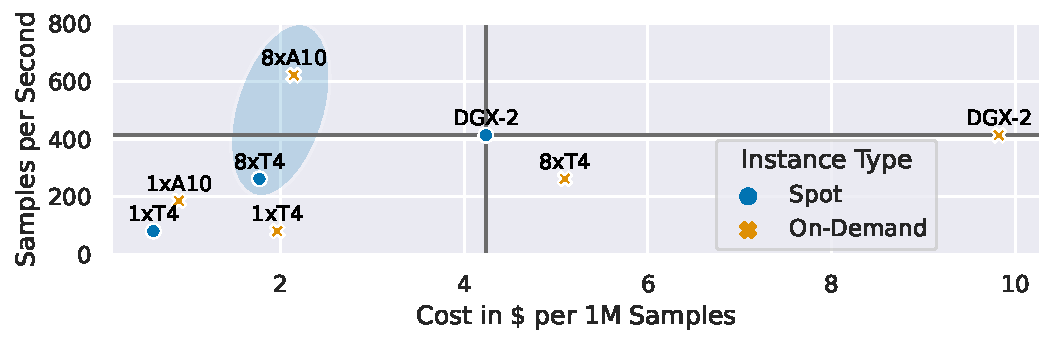
\includegraphics[width=0.49\textwidth]{figures/misc/cv_cost_per_sps_comparison}
    \vspace{-20pt} 
    \caption{Tradeoff between cost per sample (x-axis) and model throughput (y-axis) for ConvNextLarge at different instance types. Our training setups (circled) are cheaper (8xT4) and faster (8xA10) than the centralized offering (DGX-2).} 
    \label{fig:cv-sps-trade-off}
    \vspace*{-5mm} 
\end{figure} 
The single node (1xT4, 1xA10, DGX-2) experiments show the current state-of-the-art cost-throughput ratio for training on GC and LambdaLabs.
The DGX-2 node is the fastest, with a throughput of 413~SPS, but it also costs 6.30\$/h (4.24\$/1M samples), shown by the horizontal and vertical lines.
The single-accelerator experiments (1xT4, 1xA10) have a better cost-throughput ratio (0.62\$/1M samples and 0.9\$/1M samples), but have a much lower throughput of 80 and 185~SPS, respectively.
However, when using our approach of distributing the training between multiple GPUs with Hivemind (circled), we make training possible that is both faster (8xA10, 621~SPS, 2.15\$/1M samples) and cheaper (8xT4, 262~SPS, 1.77\$/1M samples) than using the DGX-2.
Every cloud provider deals differently with how they price spot instances and network traffic (cf.~\Cref{tab:cloud-pricing}) and has varying interruption rates for different accelerators~\cite{lee2017deepspotcloud}.
Being able to choose the best option was not possible before, and having the option to combine older, more available GPUs is a net benefit for both consumers and cloud providers alike.
 
We aim to develop guidelines and help practitioners assess under which conditions they can cost-efficiently speed up their training tasks with spot instances.
To be able to do this, they need a precise definition of the model size at which geo-distributed spot training becomes viable, what hardware can be used for it, and what the minimum bandwidth and latency are.
We close this research gap by performing a comprehensive analysis of multiple DL tasks from CV and NLP, breaking down how time is spent in each epoch, and comparing them to non-distributed runs to quantify the advantages and disadvantages of distributed spot training.
We determine which models scale with additional spot instances and which cannot be scaled without running into a communication bottleneck or resource inefficiencies.
To quantify total training cost, we assess cost-effectiveness and evaluate a hybrid or multi-cloud approach with popular cloud providers through training on up to four continents.
For comparison of the models' scalability and to show which of them can be trained in a distributed fashion, we introduce the \textit{granularity metric}, the ratio of calculation to communication time, and show how it can be used for predicting performance with different hardware setups.
Finally, we summarize our lessons on how to design geo-distributed spot training and what to watch out for when evaluating the feasibility of such a training regime. Our contributions are:
\hyphenation{dis-tri-bu-ted}
\begin{enumerate}
    \item \textbf{We analyze the impact of multi-cloud training with spot and on-demand instances from Google Cloud (GC), Microsoft Azure, Amazon Web Services (AWS), and LambdaLabs on cost-efficiency.} While we find performance penalties due to remote versus on-premise compute resources, the throughput still scales with increased computing power. By leveraging multiple spot instances with one T4 GPU each, we can be more cost-efficient than a DGX-2 node or the very competitively priced A10 offerings from LambdaLabs.
    \item \textbf{We investigate the suitability of geo-distributed training for various CV and NLP models and hardware configurations on up to four continents.} Not surprisingly, the more parallelizable and the larger the task, the better the performance. Moreover, we verify the scalability claims of the related work and define additional constraints, such as the minimum granularity for effective training. This enables, for the first time, distributed training speeds of smaller million-parameter models (12M-560M) over <1~Gbits bandwidth and >150ms latency networks.
    \item \textbf{We evaluate two different hybrid-cloud experimental setups with consumer- and server-grade on-premise hardware} and try to improve the throughput with a bandwidth of, at worst, 50~Mbits to the cloud resources. While we show that it is possible to improve throughput even at these connectivity constraints, local cloud offerings are better suited for models that show limited suitability for distributed training.
    \item We summarize our findings of training in a geo-distributed, multi-cloud environment. \textbf{We propose the granularity metric to compare model suitability for distributed spot training} and estimate training performance with additional spot VMs. This provides guidance on the trade-off between performance and cost when using geo-distributed spot instances.
\end{enumerate}

Our paper is organized as follows.
In ~\Cref{sec:distributed-dl}, we introduce distributed deep learning on spot instances and how the Hivemind framework enables this experimental setup.
We evaluate a comprehensive set of models on their suitability for distributed spot training in ~\Cref{sec:model-suitability}.
After selecting suitable models, we analyze the geo-distributed experiments in ~\Cref{sec:geodistributed-performance}.
Next, in ~\Cref{sec:multicloud-performance}, we evaluate the multi-cloud experiments with GC, AWS, and Azure.
Following are the hybrid-cloud experiments in ~\Cref{sec:hybrid-cloud-performance}.
Further insights and cost analysis are covered in ~\Cref{sec:further-insights}.
Our derived lessons are summarized in ~\Cref{sec:lessons-learned}.
Related work is reviewed in ~\Cref{sec:related-work}.
Finally, we conclude the paper in ~\Cref{sec:conclusion}.